\documentclass{article}
\pagenumbering{arabic}
\newcommand{\newCommandName}{text to insert}
% Pages and colors used for the cover page
\usepackage{tikz-page}
\usepackage{url}
\usepackage{lastpage}

% Used for the math and code
\usepackage{amsmath}
\usepackage{listings}
\usepackage{pythonhighlight} % Got this from github! https://github.com/olivierverdier/python-latex-highlighting/blob/master/pythonhighlight.sty

% Used for the pictures
\usepackage{float}
\usepackage{graphicx}

% For the table
\usepackage[utf8]{inputenc}

\usepackage[
  top=2cm,
  bottom=2cm,
  left=3cm,
  right=2cm,
  headheight=17pt, % as per the warning by fancyhdr
  includehead,includefoot,
  heightrounded, % to avoid spurious underfull messages
]{geometry} 

% Page numbers/header
\usepackage{fancyhdr}
\definecolor{brickred}{rgb}{0.8, 0.25, 0.33}
\definecolor{cobalt}{rgb}{0.0, 0.28, 0.67}
\definecolor{cadetgrey}{rgb}{0.57, 0.64, 0.69}

% Defining the text box being used for DEPT OF ENG
\tikzset{
        secnode/.style={
                minimum height = .16in,
                minimum width = 4.16in,
                inner xsep = 2pt,
                anchor=north east,
                draw=cadetgrey,
                fill=white,
                text=brickred,
                },
        }


         
\pagestyle{plain}
\renewcommand{\headrulewidth}{0pt}
\begin{document}


% Put name data and assignment number here
\newcommand\personaldate{February 3, 2024}
\newcommand\myname{Leo Berman}
\newcommand\myemail{leo.berman@temple.edu}
\newcommand\hwnum{02}
\newcommand\mynameabbrev{L. Berman}
\newcommand\assignmenttitle{Bayesian Decision Theory}
\newcommand\yourclass{ECE 8527: Machine Learning and Pattern Recognition}
\begin{titlepage}
	% Drawing the border and the text box 
	\newcommand{\tikzpagelayout}{
		\draw[line width = .04in,
			color = cobalt]
		($(current page.north west)+(1in,-1in)$)
		rectangle ($(current page.south east)+(-.625in,1in)$);

		\draw[line width = .04in,
			color = brickred]
		($(current page.north west)+(.92in,-.92in)$)
		rectangle ($(current page.south east)+(-.705in,1.08in)$);
		\node[secnode] at ($(current page.north west)+(6in,-.875in)$) {\small{\textbf{DEPARTMENT OF ELECTRICAL AND COMPUTER ENGINEERING}}};
	}

	\begin{center}
		\large{Homework Assignment No. \hwnum:}\break
		\break
		\large{\textbf{HW No. \hwnum: \assignmenttitle}}\break
		\break
		\large{submitted to:}\break
		\break
		\large{Professor Joseph Picone}\break
		\large{ECE 8527: Introduction to Pattern Recognition and Machine Learning}\break
		\large{Temple University}\break
		\large{College of Engineering}\break
		\large{1947 North 12th Street}\break
		\large{Philadelphia, Pennsylvania 19122}\break
		\break
		\large{\personaldate}\break
		\break
		\large{prepared by: }\break
		\break
		\large{\myname}\break
		\large{Email: \myemail}
	\end{center}
\end{titlepage}

\newpage
\pagestyle{fancy}
\fancyhead{}
\fancyfoot{}
\fancyhead[R,EH]{Page \thepage\ of \pageref{LastPage}}
\fancyhead[L,EH]{\mynameabbrev: HW \# \hwnum}
\fancyfoot[L,EF]{\yourclass}
\fancyfoot[R,EF]{\personaldate}
\renewcommand{\thesection}{\Alph{section}.}

\section{\MakeUppercase{Generate multivariate Gaussian distributions}}
\large{Generate multivariate Gaussian distributions with a mean vector of zero and covariances matrices :}
\[
(A)\begin{bmatrix} 
        1 & 0\\
        0 & 1
\end{bmatrix}
(B)\begin{bmatrix} 
        5 & 0\\
        0 & 2
\end{bmatrix}
(C)\begin{bmatrix} 
        2 & 0\\
        0 & 5
\end{bmatrix}
(D)\begin{bmatrix} 
        1 & .5\\
        .5 & 1
\end{bmatrix}
(E)\begin{bmatrix} 
        1 & -.5\\
        -.5 & 1
\end{bmatrix}
(F)\begin{bmatrix} 
        5 & .5\\
        .5 & 2
\end{bmatrix}
(G)\begin{bmatrix} 
        5 & -5\\
        -.5 & 2
\end{bmatrix}
\]
\break\break
In order to generate these covariance's and plot their eigenvectors I used the following matlab script.
\begin{python}
        # Import relevant libraries
        import numpy
        import pandas
        import matplotlib.pyplot as plt

        # generate multivariate guassians
        def GMG(mean,cov,nelem):
            return numpy.random.multivariate_normal(mean,cov,nelem)
        
        # calculate eigenvectors
        def CE(inmat):
            return numpy.linalg.eig(inmat)
        
        def main():
            # number of elements
            number_elements = 5000
        
           # declare mean for all covariance matrixes
            mean = [0,0]
        
            # declare covariance matrixes
            cov_0 = [[1,0],[0,1]]
            cov_1 = [[5,0],[0,2]]
            cov_2 = [[2,0],[0,5]]
            cov_3 = [[1,.5],[.5,1]]
            cov_4 = [[1,-.5],[-.5,1]]
            cov_5 = [[5,.5],[.5,2]]
            cov_6 = [[5,-.5],[-.5,2]]
        
            # concatenate all covariance matrixes into a list
            cov_list = [cov_0,cov_1,cov_2,cov_3,cov_4,cov_5,cov_6]
        
            # declare list for points to go into
            points_list = []
        
            # declare list of eigenvectors and eIgenvalues
            eigenvectors_list = []
            eigenvalues_list = []
        
            # Colors list
            colors_list = ['r','b','y','g','o']
        
            # Generate guassians for allcovariance matrixes
            for i in range(len(cov_list)):
                # Generate Guassian points
                points_list.append(GMG(mean,cov_list[i],number_elements))
                
                # Plot the points
                plt.plot(points_list[i][:,0], points_list[i][:,1], '.', alpha = 0.5, zorder = 0)
                
                # Calculate covariance matrix eigenvectors and eigenvalues
                eigenvalues,eigenvectors = CE(cov_list[i])
                eigenvectors_list.append(eigenvectors)
                eigenvalues_list.append(eigenvalues)
        
                # Plot the eigenvectors
                for j in range(len(eigenvectors)):
                    print(eigenvalues[j])     
                    plt.quiver(*mean, *(eigenvectors[:,j]*eigenvalues[j]), scale = 18, color = colors_list[j], zorder = 10)
                
                # Plot the rest of the points and save it as a png
                plt.xlim(-10,10)
                plt.ylim(-10,10)
                plt.grid()
                #plt.show()
                plotname = "Cov_" + str(i) + ".png"
                plt.savefig(plotname)
                plt.clf()
                plt.cla()
               
        main()

\end{python}
\pagebreak
\begin{flushleft}
As expected, the diagonal of the Covariance Matrices is expressed by the covariances (anti-diagonal of matrix) and the spread in the vertical or horizontal directions is expressed by the variances(diagonal of the matrix).\break
\break
For example, in Figure 7 there is a large spread in the horizontal direction so we can expect that the Matrix[0][0] element is going to be high. If we refer back to Matrix G we can see that the number is 5 which is significantly higher .
\end{flushleft}
\begin{figure}[!htb]
        \centering
        \begin{minipage}{0.24\textwidth}
                \centering
                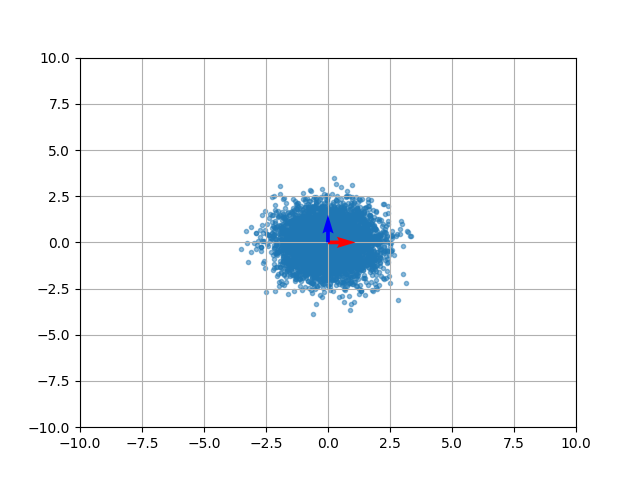
\includegraphics[width=1\linewidth]{../Cov_0.png}
                \caption{(A)}
        \end{minipage}\hfill
        \begin{minipage}{0.24\textwidth}
                \centering
                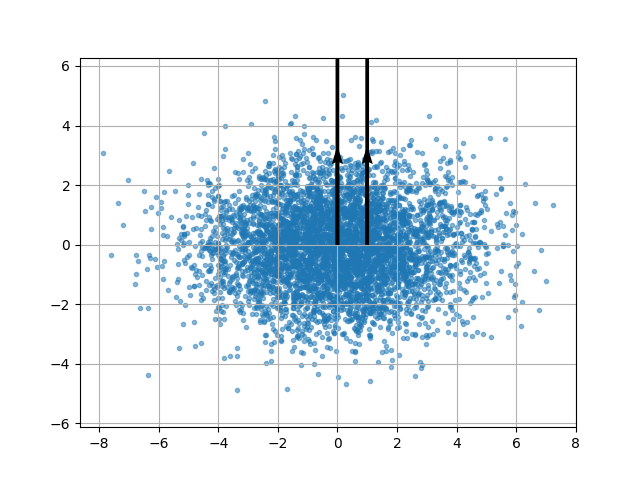
\includegraphics[width=1\linewidth]{../Cov_1.png}
                \caption{(B)}
        \end{minipage}
        \begin{minipage}{0.24\textwidth}
        \centering
                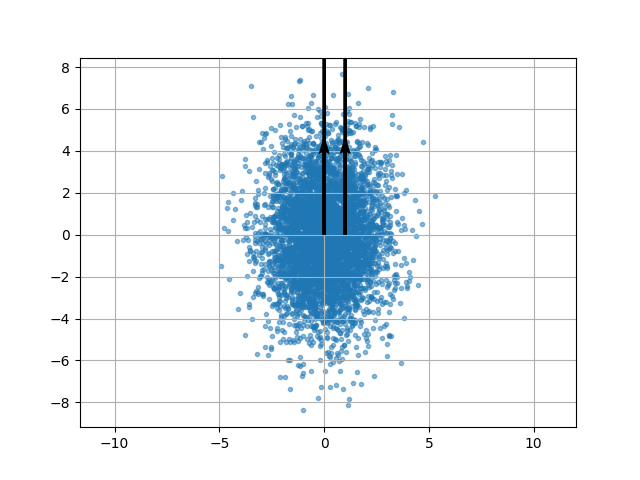
\includegraphics[width=1\linewidth]{../Cov_2.png}
                \caption{(C)}
        \end{minipage}\hfill
        \begin{minipage}{0.24\textwidth}
                \centering
                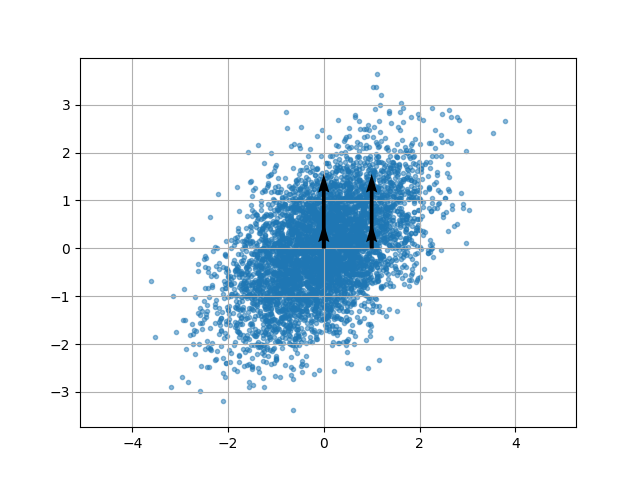
\includegraphics[width=1\linewidth]{../Cov_3.png}
                \caption{(D)}
        \end{minipage}
\end{figure}
\begin{figure}[!htb]
        \centering
        \begin{minipage}{0.24\textwidth}
                \centering
                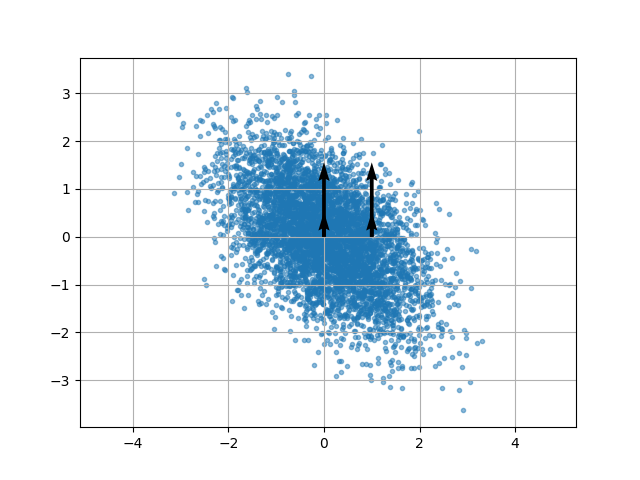
\includegraphics[width=1\linewidth]{../Cov_4.png}
                \caption{(E)}
        \end{minipage}
        \begin{minipage}{0.24\textwidth}
                \centering
                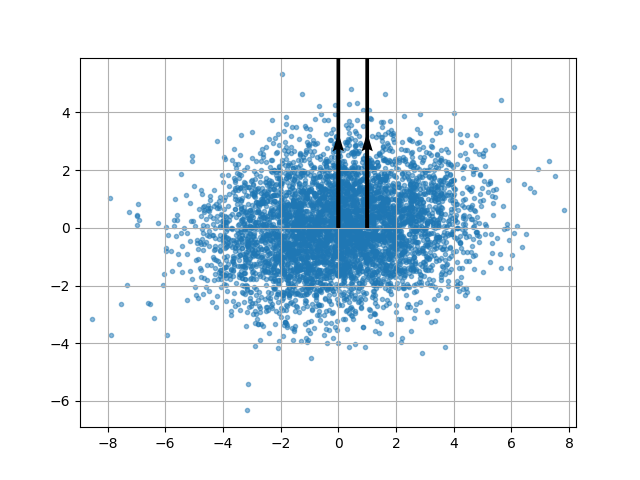
\includegraphics[width=1\linewidth]{../Cov_5.png}
                \caption{(F)}
        \end{minipage}
        \begin{minipage}{0.24\textwidth}
        \centering
                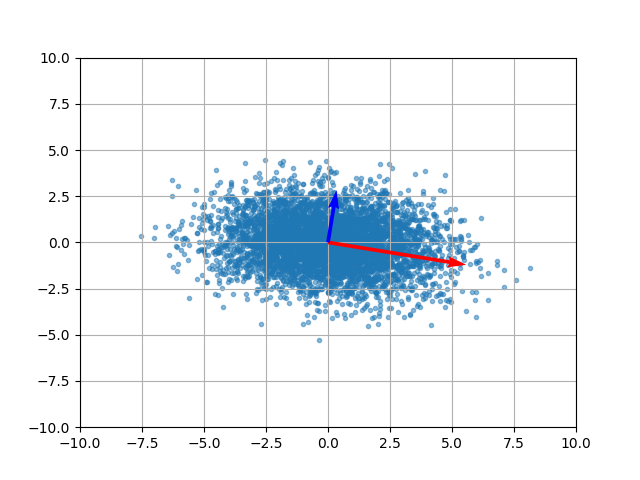
\includegraphics[width=1\linewidth]{../Cov_6.png}
                \caption{(G)}
        \end{minipage}
\end{figure}
\pagebreak
\section{\MakeUppercase{Generate QDA on multiple analysis platforms}}
\begin{flushleft}
\textbf{IMLD}\break
\break
First, the proprietary software IMLD was used to get a base to compare from. When trained on the train.csv data from data set 13, the train.csv data had an error rate of 11.39\%\, and the eval.csv data had an error rate of 20.49\%\. \break
\break
IMLD's visualization of the decision surfaces:\break
\begin{figure}[!htb]
        \centering
        \begin{minipage}{0.49\textwidth}
                \centering
                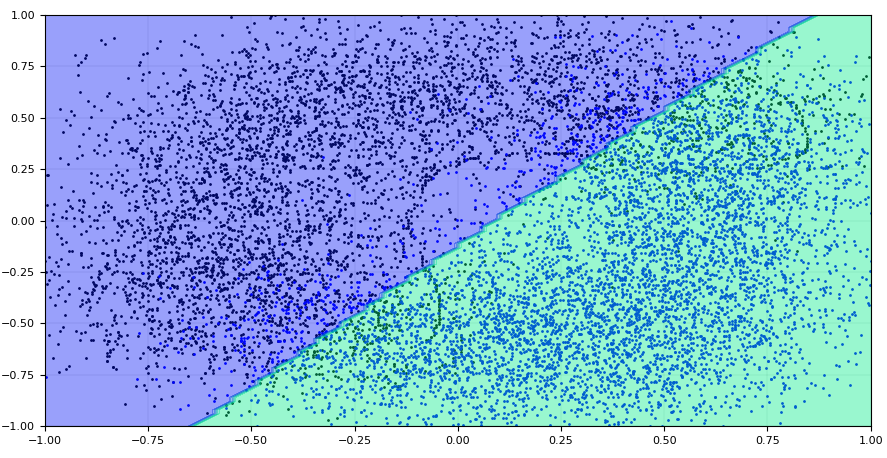
\includegraphics[width=1\linewidth]{../IMLDTrain.png}
                \caption{Training Dat}
        \end{minipage}
        \begin{minipage}{0.49\textwidth}
                \centering
                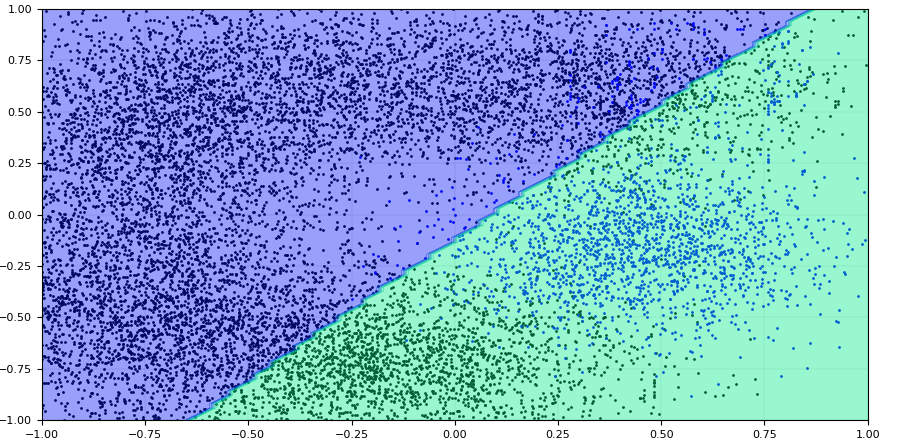
\includegraphics[width=1\linewidth]{../IMLDEval.png}
                \caption{Evaluation Data}
        \end{minipage}
\end{figure}
\break
\textbf{JMP}\break
\break
Next, the data was processed in the program JMP which uses a validation column process/notation. The model was trained on train.csv from data set 13 and validated using eval.csv from the same data set. The data train.csv had an error rate of 11.34\%\ and the validation data from eval.csv had an error rate of 21.31\%\break
\break
JMP's visualization using a canonical plot which is another plot type to show the correlation of two sets of variables:\break
\begin{figure}[!htb]
        \centering
        \begin{minipage}{0.49\textwidth}
                \centering
                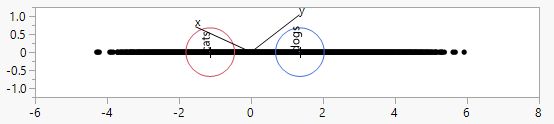
\includegraphics[width=1\linewidth]{../JMPCanonicalPlot.png}
                \caption{Canonical Plot of QDA Model}
        \end{minipage}
\end{figure}
\pagebreak
\textbf{SKLearn}\break
\break
Next, the data was processed using SKLearn's QDA model which resulted in a train.csv error rate of 11.11\%\ and a eval.csv error rate of 20.83\%.\break
\break
This is the implimentation using SKLearn's QDA model:\break
\begin{python}
from sklearn.discriminant_analysis import QuadraticDiscriminantAnalysis as QDA
import numpy as np
import pandas as pd
import sys
def main():
        # read in the data from the csv files
        train = pd.read_csv("train.csv",comment = "#").to_numpy()
        eval = pd.read_csv("eval.csv", comment = "#").to_numpy()
        train_coords = np.array(list(zip(train[:,1],train[:,2])))
        eval_coords = np.array(list(zip(eval[:,1],eval[:,2])))
        
        # Set and train the algorithm
        algo = QDA()
        algo.fit(train_coords,train[:,0])
        
        # Evaluate the algorithm
        print("Evaluation accuracy rate: ",1-algo.score(eval_coords,eval[:,0]))
        print("Training accuracy rate: ",1-algo.score(train_coords,train[:,0]))
        
        
main()
\end{python}
\pagebreak
\textbf{Custom Implimentation}\break
\break
The custom implimentation resulted in a train.csv error rate of 11.12\%\, and an eval.csv error rate of 20.83\%.\break
\break
This is the custom implimentation:\break
\begin{python}
# Import relevant values       
import numpy as np
import pandas as pd
import sys
class Classifier:

        # initialize values
        def __init__(self,inname):
                self.class_name =       inname
                self.number_elements =  0
                self.x_mean =           None
                self.y_mean =           None
                self.x_sd =             None
                self.y_sd =             None
                self.data =             np.array([])
                self.cov =              None
                self.cov_mat =          None
                self.x_var =            None
                self.y_var =            None
                self.mean_vec =         None

        # Add in Classifier data
        def add_data(self,indata):
                if len(self.data) == 0:
                        self.data = indata
                else:
                        self.data=np.vstack([self.data, indata])
                        self.number_elements+=1
        
        # Calculating the mean of each Classifier of the class
        def calculate_mean(self):
                x_sum = 0
                y_sum = 0
                for x in self.data:
                        x_sum+=x[0]
                        y_sum+=x[1]
                self.x_mean = x_sum/self.number_elements
                self.y_mean = y_sum/self.number_elements
        
        # calculate mean_vector
        def calculate_mean_vector(self):
                self.calculate_mean()
                self.mean_vec = np.array([self.x_mean,self.y_mean])
        
        # Calculating covariance
        def calculate_covariance(self):
                work = 0
                for x in self.data:
                        work+=(x[0] - self.x_mean) * (x[1] - self.y_mean)
                self.cov = work / (self.number_elements-1)
        
        # Calculating covariance matrix
        def calculate_covariance_matrix(self):
                self.calculate_covariance()
                self.calculate_variance()
                self.cov_mat = np.array([[self.x_var, self.cov],[self.cov, self.y_var]])

        # Calculating variance
        def calculate_variance(self):
                x_sum = 0
                y_sum = 0
                for x in self.data:
                        x_sum+=(x[0]-self.x_mean)**2
                        y_sum+=(x[1]-self.y_mean)**2
        
                self.x_var = x_sum/(self.number_elements-1)
                self.y_var = y_sum/(self.number_elements-1)
        
class Custom_QDA:

        # constructor
        def __init__(self):
        
                # keep track of classes
                self.classes = {}
        
                # keep track of number of elements
                self.number_elements = 0
        
                # Keeping track of totals
                self.value_totals = {}
        
        # training the model
        def train(self,training_data):
                
                # iterate through all data
                for i in range(len(training_data)):
                
                        # check if there is already a Classifier for the class if not make one
                        if training_data[i][0] not in self.classes:

                                # total values and make new Classifiers
                                self.classes[training_data[i][0]]=Classifier(training_data[i][0])
                        
                        # Add data to Classifier
                        self.classes[training_data[i][0]].add_data(np.array([float(training_data[i][1]),float(training_data[i][2])]))
                
                        # Keep track of total number of elements
                        self.number_elements+=1
                
                        # Call functions for calculating means and covariance matrix
                for x in self.classes:
                        self.classes[x].calculate_mean_vector()
                        self.classes[x].calculate_covariance_matrix()
        
        # calculate probabilities for individual classes and make a guess
        def return_probability(self,inclass,inx,iny):
                
                # No guess 0 confidence
                guess = None
                guess_prob = -1*float("inf")
                
                # Iterate through all classes and calculate each Classifiers probability density
                for x in self.classes:
                
                        # Mean vector            
                        mean_vector = self.classes[x].mean_vec
                
                        # Classifier vector
                        Classifier_vector = np.array([inx,iny])
                
                        # Covariance matrix
                        covariance_matrix = self.classes[x].cov_mat
                        
                        # Elements for calculating naive bayes score
                        ele1_1 = np.matmul(np.transpose(Classifier_vector-mean_vector),np.linalg.inv(covariance_matrix))
                        ele1_2 = Classifier_vector-mean_vector
                        ele1 = -.5 * np.matmul(ele1_1,ele1_2)
                        ele2 = -.5 * np.log(2*np.pi)
                        ele3 = -.5 * (np.log(np.linalg.det(covariance_matrix)))
                        ele4 = np.log(self.classes[x].number_elements/self.number_elements)
                
                        # Calculate naive bayes score
                        total_prob = ele1 + ele2 + ele3 + ele4
                
                        # If probability is greater than last guess set as new guess
                        if total_prob > guess_prob:
                                guess_prob = total_prob
                                guess = x
                
                # Check to see if guess was correct or incorrect
                if guess == inclass:
                        return True
                else:
                        return False
        
        # Evaluate data
        def eval(self,newdata):
                
                # Keep track of guesses and return the correct/total
                total_correct = 0
                total = 0
                for x in newdata:
                        total +=1

                        # Call the return p robability function which guesses and returns True 

                        # When correct and False when not
                        if (self.return_probability(x[0],float(x[1]),float(x[2]))) == True:
                                total_correct += 1

                # calculate accuracy_rate
                accuracy_rate = total_correct/total
                return accuracy_rate
        
def main():

        # read data in and turn it into a 3 column numpy array
        train = pd.read_csv("train.csv",comment = "#").to_numpy()
        eval = pd.read_csv("eval.csv", comment = "#").to_numpy()
        train = np.array(list(zip(train[:,0],train[:,1],train[:,2])))
        eval = np.array(list(zip(eval[:,0],eval[:,1],eval[:,2])))

        # initialize model
        my_QDA = Custom_QDA()
        my_QDA.train(train)
        
        # print the results from the evaluations
        print("Evaluation accuracy rate = ", 1-my_QDA.eval(eval))
        print("Training accuracy rate = ", 1-my_QDA.eval(train))
main()
\end{python}
\end{flushleft}
\textbf{Results Summary Table}\break
\break
\begin{center}
\begin{tabular}{c c c c c c c c c}
        a & b & c & d & e & f & g & h & 9\\
\end{tabular}
\end{center}
\textbf{Why aren't these numbers the same?}\break
\break

\section{SUMMARY}
\large{Briefly describe what you learned from this assignment and ways you could improve your solutions.}
\end{document}